\subsection{Experiment 5: Characteristics of Metrics in Classification Tasks}

\begin{figure}[H]
    \centering
    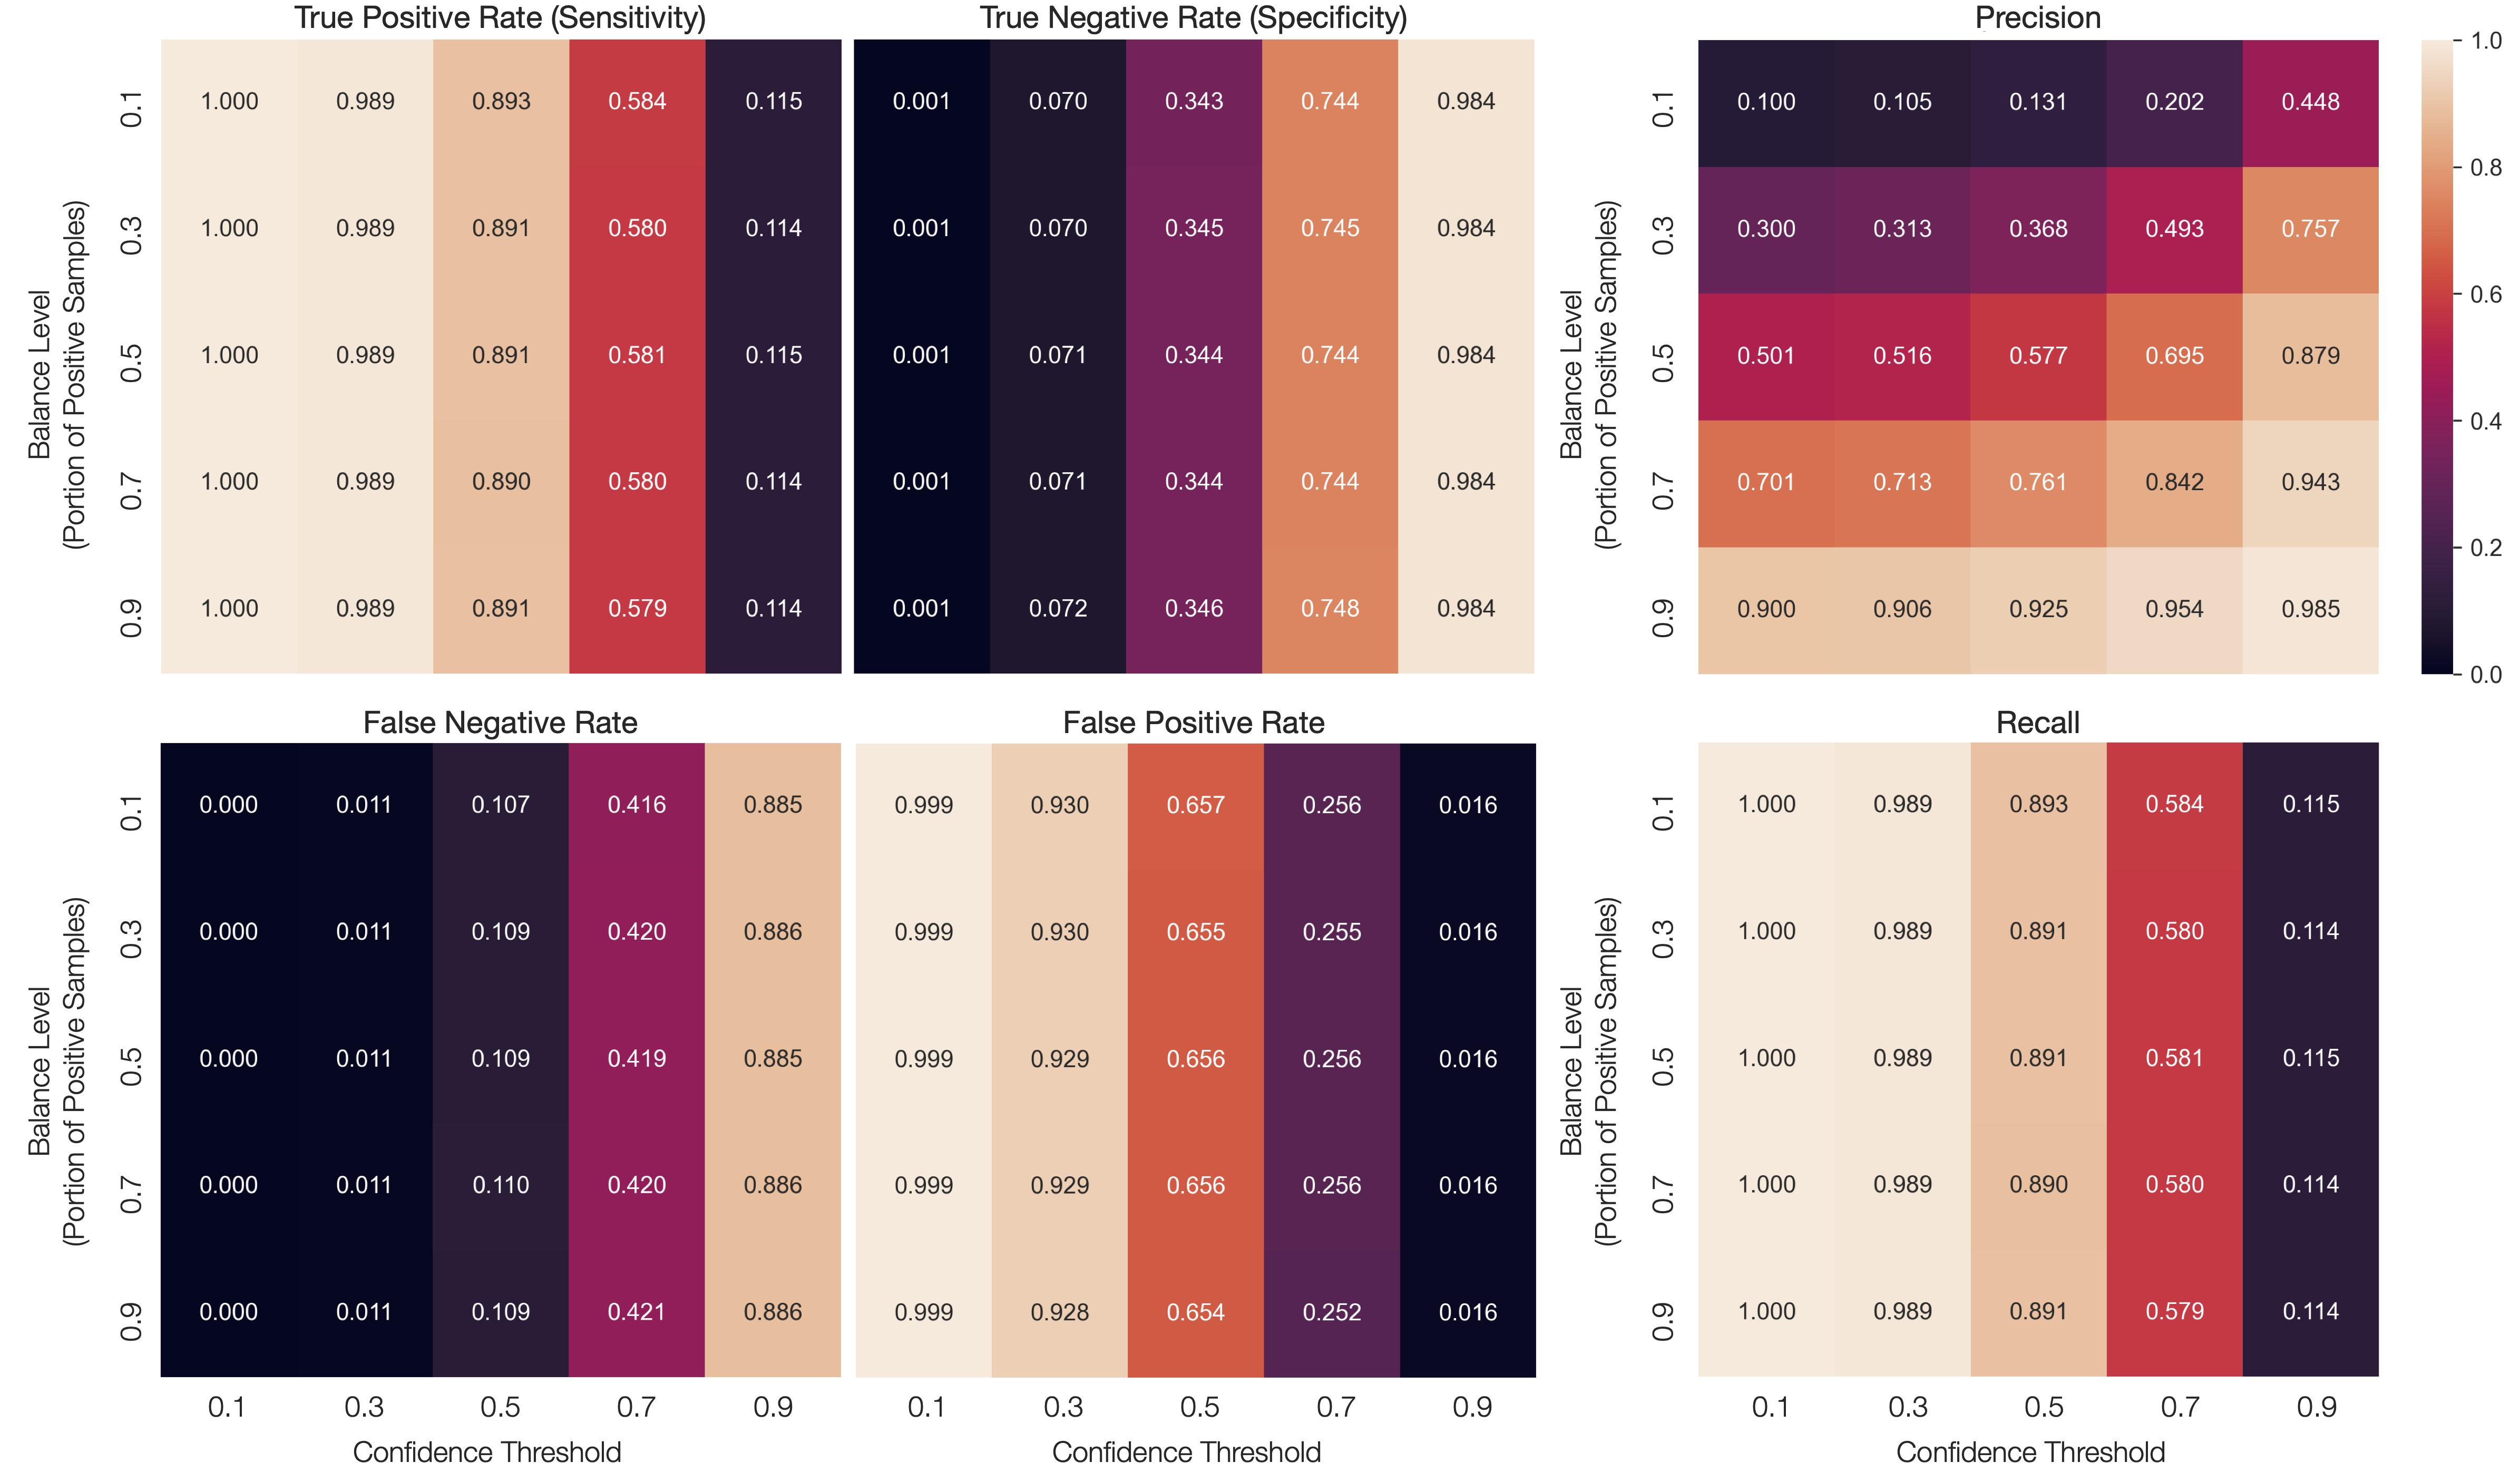
\includegraphics[width=1\textwidth]{fig_10.jpg}
    \caption{Heatmaps displaying performance metrics across a 5×5 grid, where each cell corresponds to a unique combination of balance level and confidence threshold. These metrics are calculated exclusively for either positive or negative class label. The simulation is configured such that the model produces more false positive than false negative predictions, with the negative class following a beta distribution ($\alpha = 4, \beta = 3$).} 
    \label{fig:s5_1}
\end{figure}

Except for precision, metrics focused on a single sample distribution (i.e., actual positives or negatives) are unaffected by class imbalance (Figure~\ref{fig:s5_1}). For instance, the TPR remains stable at 0.989 with a confidence threshold of 0.3, regardless of the proportion of positive samples. This stability arises because such metrics evaluate only one distribution at a time, making them invariant to shifts in class balance.

To capture a more comprehensive view of model performance, multiple metrics are often combined. In this experiment, where false positives are more frequent than false negatives, TPR alone is insufficient, as it focuses only on actual positives. Including TNR accounts for false positives among actual negatives, revealing the model’s overall tendency to produce more false positives than false negatives. Since TNR and FPR (false positive rate) are complementary (TNR + FPR = 1), as are TPR and FNR (false negative rate), these pairs offer flexibility in reporting and interpreting classification errors. Researchers can choose to emphasize either the correctness (TPR and TNR) or error (FPR and FNR) aspects of model predictions, depending on the application context.

In agricultural disease diagnosis, both TPR (sensitivity) and TNR (specificity) are critical for evaluating performance. These metrics ensure accurate identification of both positive (diseased) and negative (healthy) cases. For example, Buczinski et al. (2018) used biometric indicators to detect bovine respiratory disease \citep{buczinski_validation_2018}, while Lu et al. (2017) relied on camera images to identify wheat stripe rust and black chaff \citep{lu_-field_2017}. These studies highlight the importance of sensitivity and specificity for balanced evaluations in diagnostic applications.

In contrast, precision and recall focus on predicted positive samples instead of actual positives, making them essential for tasks prioritizing prediction quality on positive samples over identifying all instances of interest. It is worth noting that precision measures the correctness of positive predictions and is highly sensitive to class imbalance and confidence thresholds. For example, in a dataset with 70\% positive samples, a naive model (i.e., when threshold = 0.1) predicting all samples as positive achieves a baseline precision of 0.7. It can only be considered modest improvement if a model reports a high precision of 0.8. However, in a dataset with only 10\% positive samples, achieving a precision of 0.448 with a high confidence threshold significantly outperforms the baseline of 0.1, demonstrating strong performance in handling imbalance even with a low value of precision in this case.

Compared to using the pair of TPR and TNR, precision and recall are particularly useful in computer vision domains like image-based weed detection \citep{zhang_automated_2019, su_advanced_2020}, where the goal is to identify weeds or economic crops, which may constitute rare positive samples, against a background of negative samples (e.g., areas with no objects of interest). In such cases, TNR and FPR are less relevant, as the focus is on the reliability of the model’s predictions (precision) and its ability to capture all positive instances of weeds or crops (recall). Similarly, in natural language processing (NLP) and information retrieval tasks \citep{gao_retrieval-augmented_2024, salemi_evaluating_2024}, precision and recall play vital roles. For example, in evaluating language models, the focus is often on how reliable the generated responses are (precision) and how many relevant responses are produced (recall). Negative samples, such as irrelevant or nonsensical outputs, are typically less of a concern compared to ensuring the relevance and completeness of positive samples. In information retrieval, where a user might submit a document containing ten key pieces of information (positive samples), the emphasis is on how many of these key pieces the system retrieves (recall) and how accurate those retrieved pieces are (precision), rather than on the proportion of irrelevant information correctly ignored (TNR).

In summary, each pair of metrics (TPR and TNR, precision and recall) offers a unique perspective on model performance. TPR (or sensitivity) and TNR (specificity) are essential for evaluating the model’s ability to correctly classify positive and negative samples, respectively, while precision and recall are indispensable metrics for scenarios where identifying and evaluating the quality of positive samples are more critical than focusing on the negative ones. These metrics are not self-explanatory but remain popular in the machine learning community due to their ability to measure the reliability and completeness of positive predictions in tasks where negative samples are of secondary interest.


\begin{figure}[H]
    \centering
    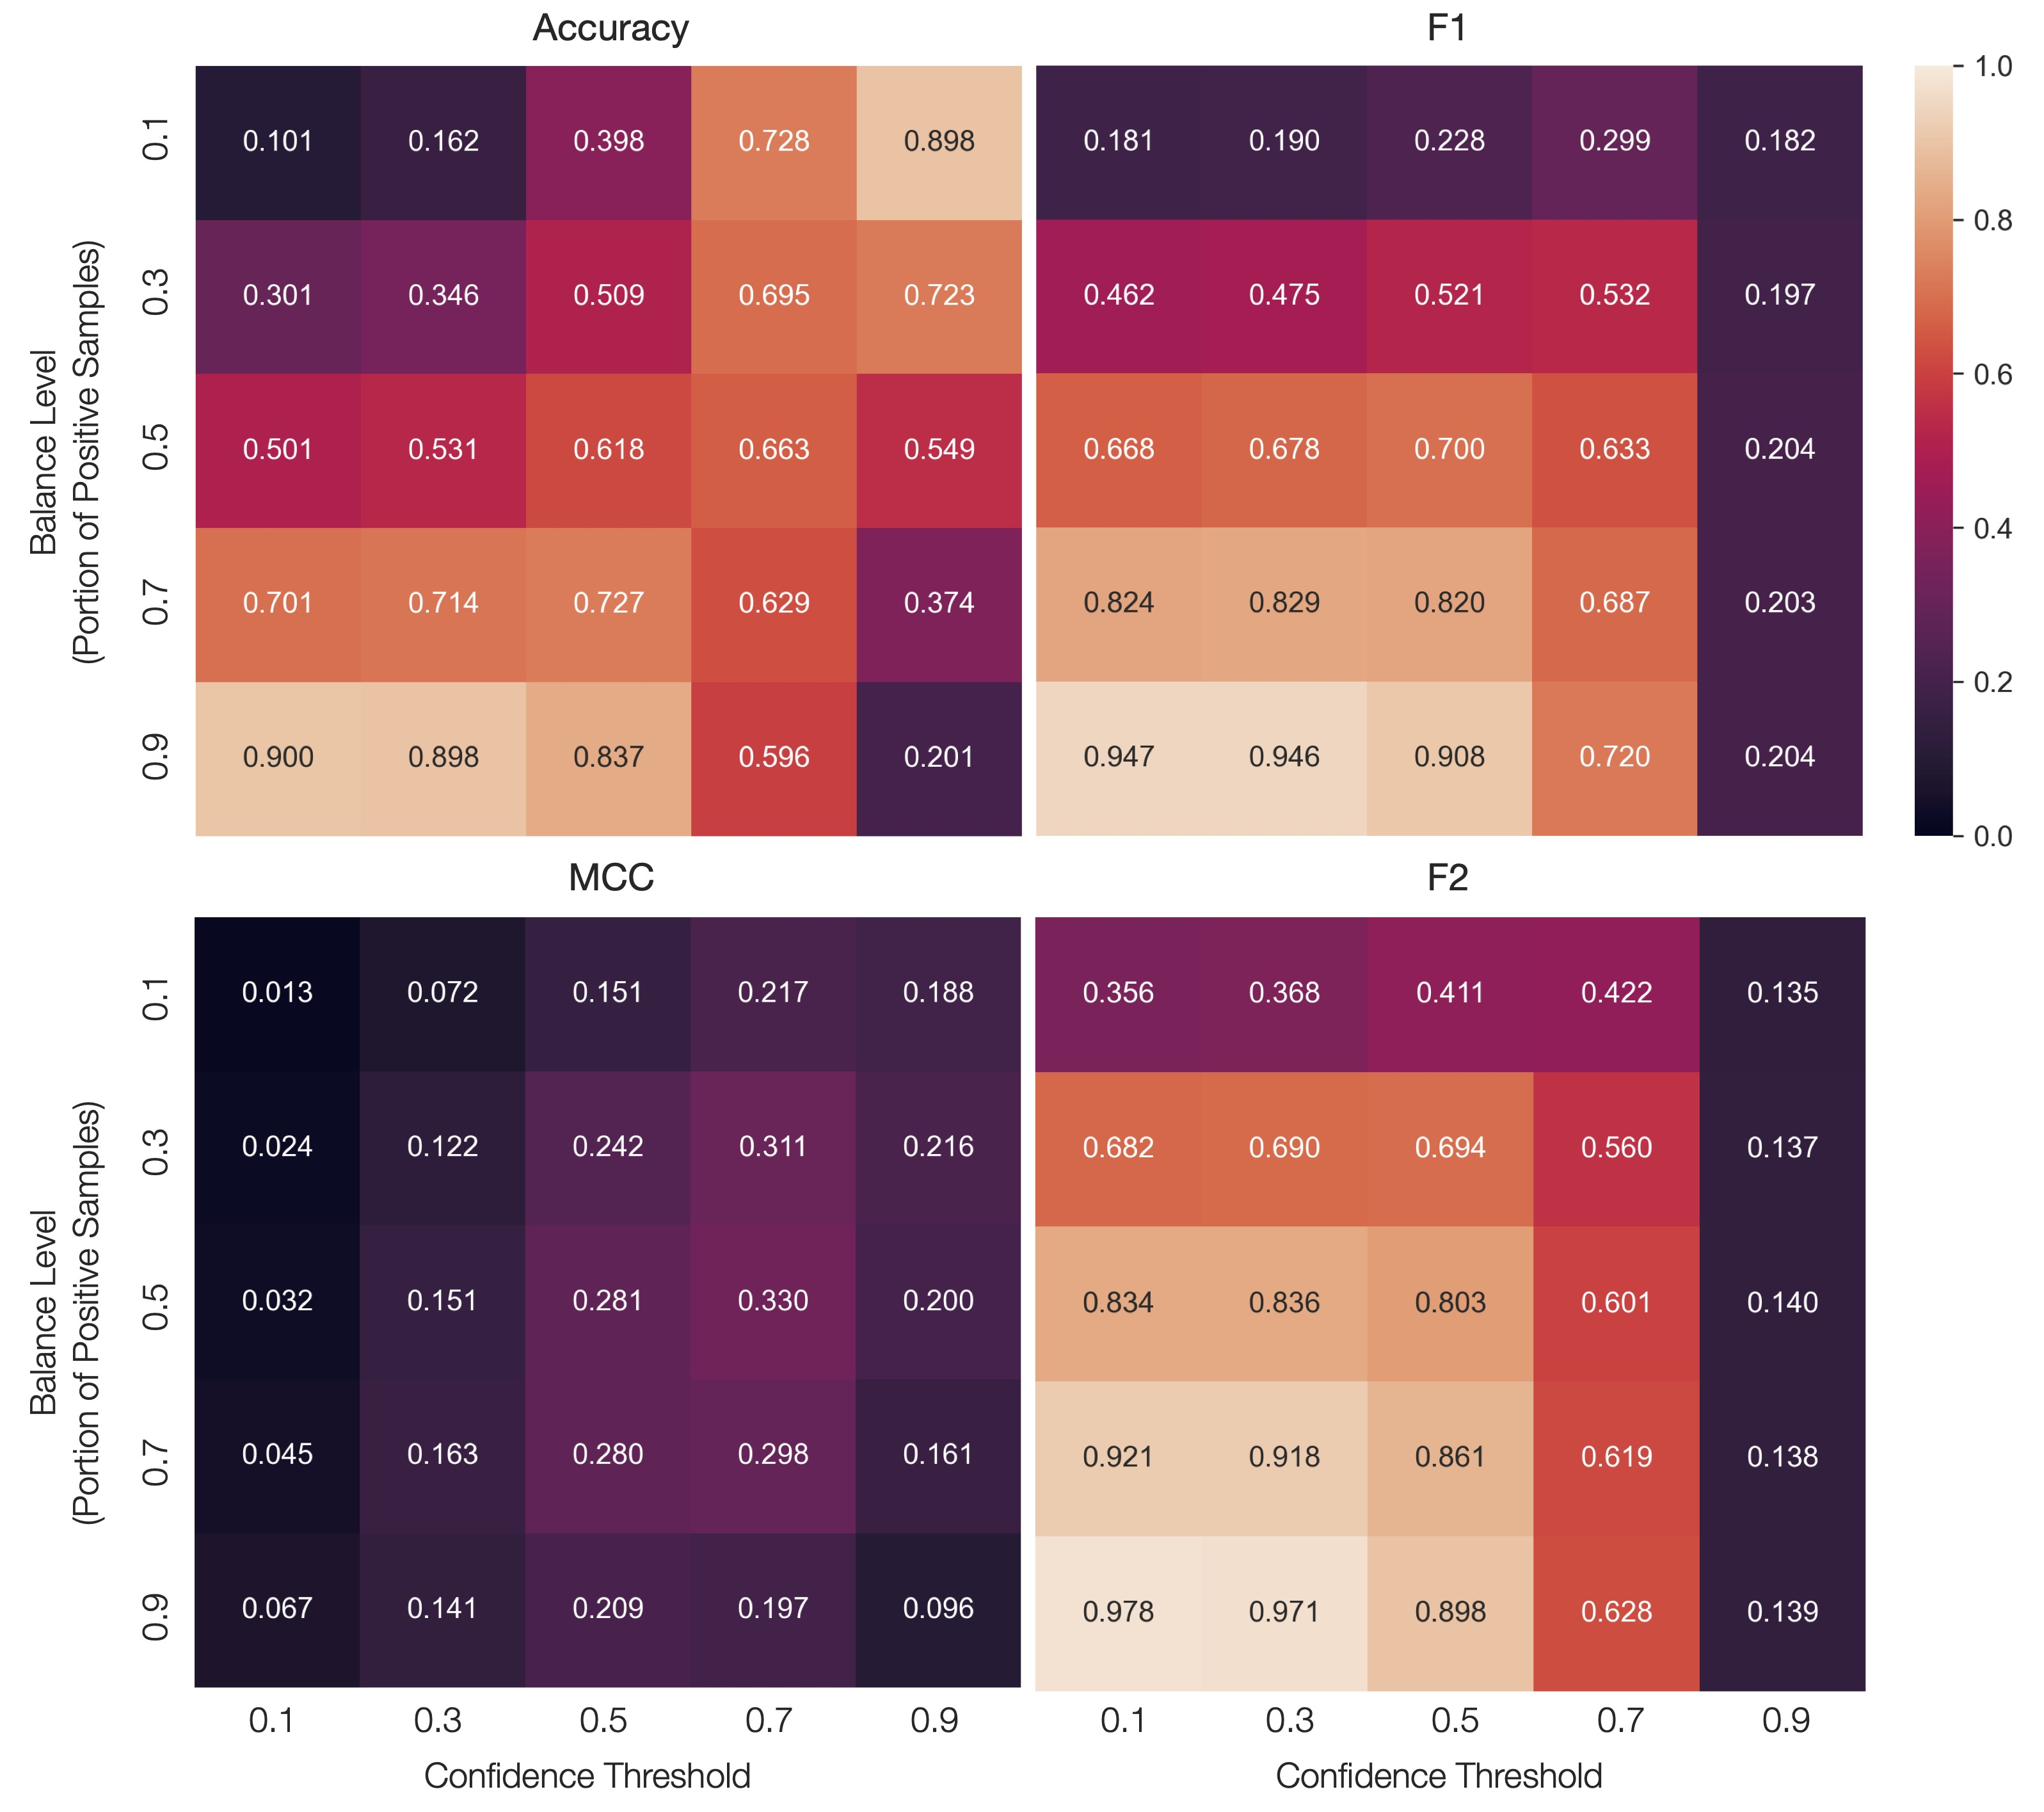
\includegraphics[width=.7\textwidth]{fig_11.jpg}
    \caption{A 5 × 5 grid of performance metrics, with each cell representing a unique combination of balance and confidence threshold. The inspected metrics focus on multiple sample distributions simultaneously. The prediction model is simulated to have higher false positive rate than false negative rate.}
    \label{fig:s5_2}
\end{figure}



Metrics that capture multiple aspects of model performance offer more comprehensive insights into a model’s effectiveness (Figure~\ref{fig:s5_2}). The heatmap in this experiment illustrates extreme scenarios at its corners, highlighting metric strengths and limitations. For example, the top-left corner features predominantly negative samples with mostly positive predictions, leading to many false positives, while the bottom-right corner features predominantly positive samples with mostly negative predictions, resulting in false negatives. The other corners illustrate cases where predictions align overwhelmingly with the majority class, allowing naive models to achieve high performance purely due to class imbalance rather than true predictive power. Effective metrics must assess performance beyond such “background effects.”

Accuracy, while simple and widely used, is limited in these extreme cases. For instance, in the top-left corner, accuracy drops due to false positives, whereas in corners dominated by a majority class, accuracy can be misleadingly high. For example, in the top-right corner, where 90\% of samples are negative, a model predicting all negatives achieves 90\% accuracy, despite ignoring true positives. Such scenarios demonstrate accuracy’s inability to capture critical trade-offs between false positives and false negatives.

The F1-score addresses accuracy’s limitations by balancing precision and TPR (i.e., recall), making it suitable for moderately imbalanced datasets. For example, in the same top-right corner of the heatmap, the F1-score of 0.182 reflects sensitivity to both false positives and false negatives, unlike accuracy, which may inflate performance due to imbalance. Real-world studies, such as Haque et al. (2023), underscore this: in a maize leaf blight detection task with a 1:2 class imbalance, an accuracy of 99.02\% masked the model’s limitations. Instead, an F1-score of 97.49\% provided a clearer measure of the model’s ability to balance precision and TPR \citep{haque_recognition_2023}.

Variants like the F2-score further refine performance evaluation by prioritizing TPR over precision, making it useful for scenarios where missing positive cases is costly. For instance, Minni (2024) applied the F2-score in breast cancer diagnosis to emphasize capturing positive cases, addressing the severe consequences of false negatives \citep{minni_exploring_2024}.

The MCC provides a robust alternative by considering all confusion matrix components and mitigating sensitivity to class imbalance. Becker et al. (2021) demonstrated MCC’s stability across datasets with varying imbalances, ranging from mildly (119 vs. 153 samples) to severely imbalanced (265 non-stress vs. 50 stress samples), when predicting heat stress in dairy cattle. Unlike F1-scores, which can reflect class distribution more than true classifier quality, MCC delivered a more comprehensive and reliable evaluation \citep{becker_predicting_2021}. These examples highlight MCC’s effectiveness in assessing model performance across diverse contexts.
